\def\pgfsysdriver{pgfsys-dvisvgm.def}
% flashcards-title: Condition returning toward a workable range after disturbance
% flashcards-desc: Three panels show a dot inside a dashed workable band, then below it after a disturbance, then back inside the band later.
\documentclass[tikz,border=6pt]{standalone}
\usetikzlibrary{arrows.meta,calc,fit,positioning,shapes.geometric}

\definecolor{fcink}{HTML}{17212B}
\definecolor{fcblue}{HTML}{1D5D8C}
\definecolor{fcgreen}{HTML}{2D6A4F}
\definecolor{fcorange}{HTML}{A44A1F}
\definecolor{fcpale}{HTML}{F4F7F9}
\definecolor{fcsoil}{HTML}{8B5E3C}

\tikzset{
  fc text/.style={font=\sffamily, text=fcink},
  fc panel/.style={draw=fcink, line width=0.9pt, rounded corners=5pt, fill=fcpale},
  fc node/.style={draw=fcink, line width=0.9pt, rounded corners=4pt, fill=white,
    minimum width=24mm, minimum height=10mm, align=center, font=\sffamily},
  fc arrow/.style={-{Stealth[length=3.2mm,width=2.4mm]}, line width=1.2pt,
    draw=fcblue, line cap=butt},
  fc boundary/.style={draw=fcorange, line width=1.4pt, dash pattern=on 5pt off 3pt,
    rounded corners=7pt},
  fc label/.style={font=\sffamily\bfseries, text=fcink},
  fc note/.style={font=\sffamily\small, text=fcink, align=center}
}

\begin{document}
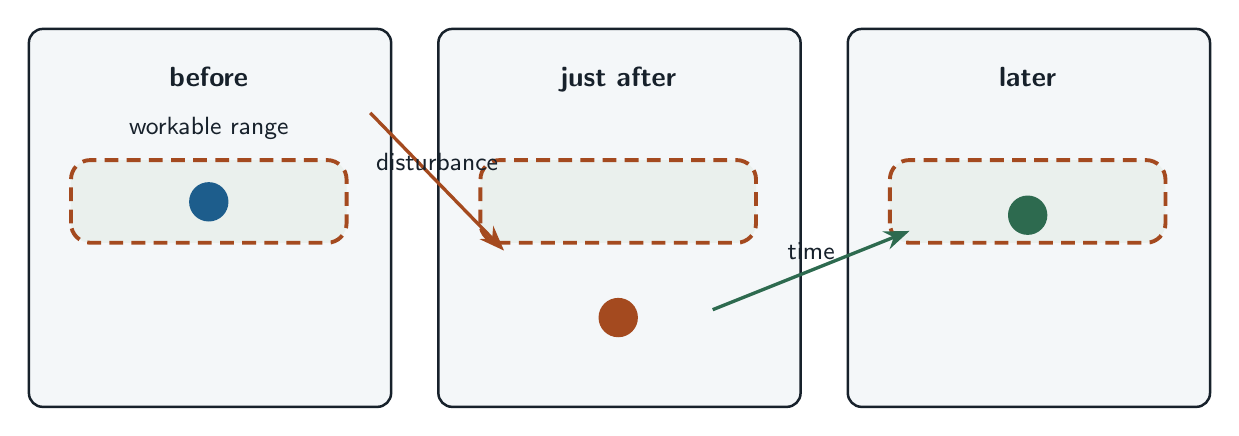
\begin{tikzpicture}[fc text, x=1cm, y=1cm]
  \foreach \x/\lab in {0/before,5.2/just after,10.4/later} {
    \node[fc panel, minimum width=46mm, minimum height=48mm, anchor=south west] at (\x,0) {};
    \node[fc label, anchor=north] at (\x+2.3,4.45) {\lab};
    \draw[fc boundary, fill=fcgreen!10] (\x+0.55,2.1) rectangle (\x+4.05,3.15);
  }
  \node[fc note] at (2.3,3.55) {workable range};
  \fill[fcblue] (2.3,2.62) circle (2.5mm);
  \fill[fcorange] (7.5,1.15) circle (2.5mm);
  \fill[fcgreen] (12.7,2.45) circle (2.5mm);
  \draw[fc arrow, draw=fcorange] (4.35,3.75) -- node[fc note, above] {disturbance} (6.05,2.0);
  \draw[fc arrow, draw=fcgreen] (8.7,1.25) -- node[fc note, above] {time} (11.2,2.25);
\end{tikzpicture}
\end{document}
